\documentclass{article}

\usepackage{graphicx}
\usepackage{tikz}
\usepackage{tikzsymbols}
\usetikzlibrary{calc,patterns,shapes.geometric}
\pagestyle{empty}
\usepackage[margin=0pt]{geometry}
\geometry{papersize={14in,12in}}

\def\centerarc[#1](#2)(#3:#4:#5){\draw[#1] ($(#2)+({#5*cos(#3)},{#5*sin(#3)})$) arc (#3:#4:#5);}

\begin{document}
	\begin{figure}
		\centering
		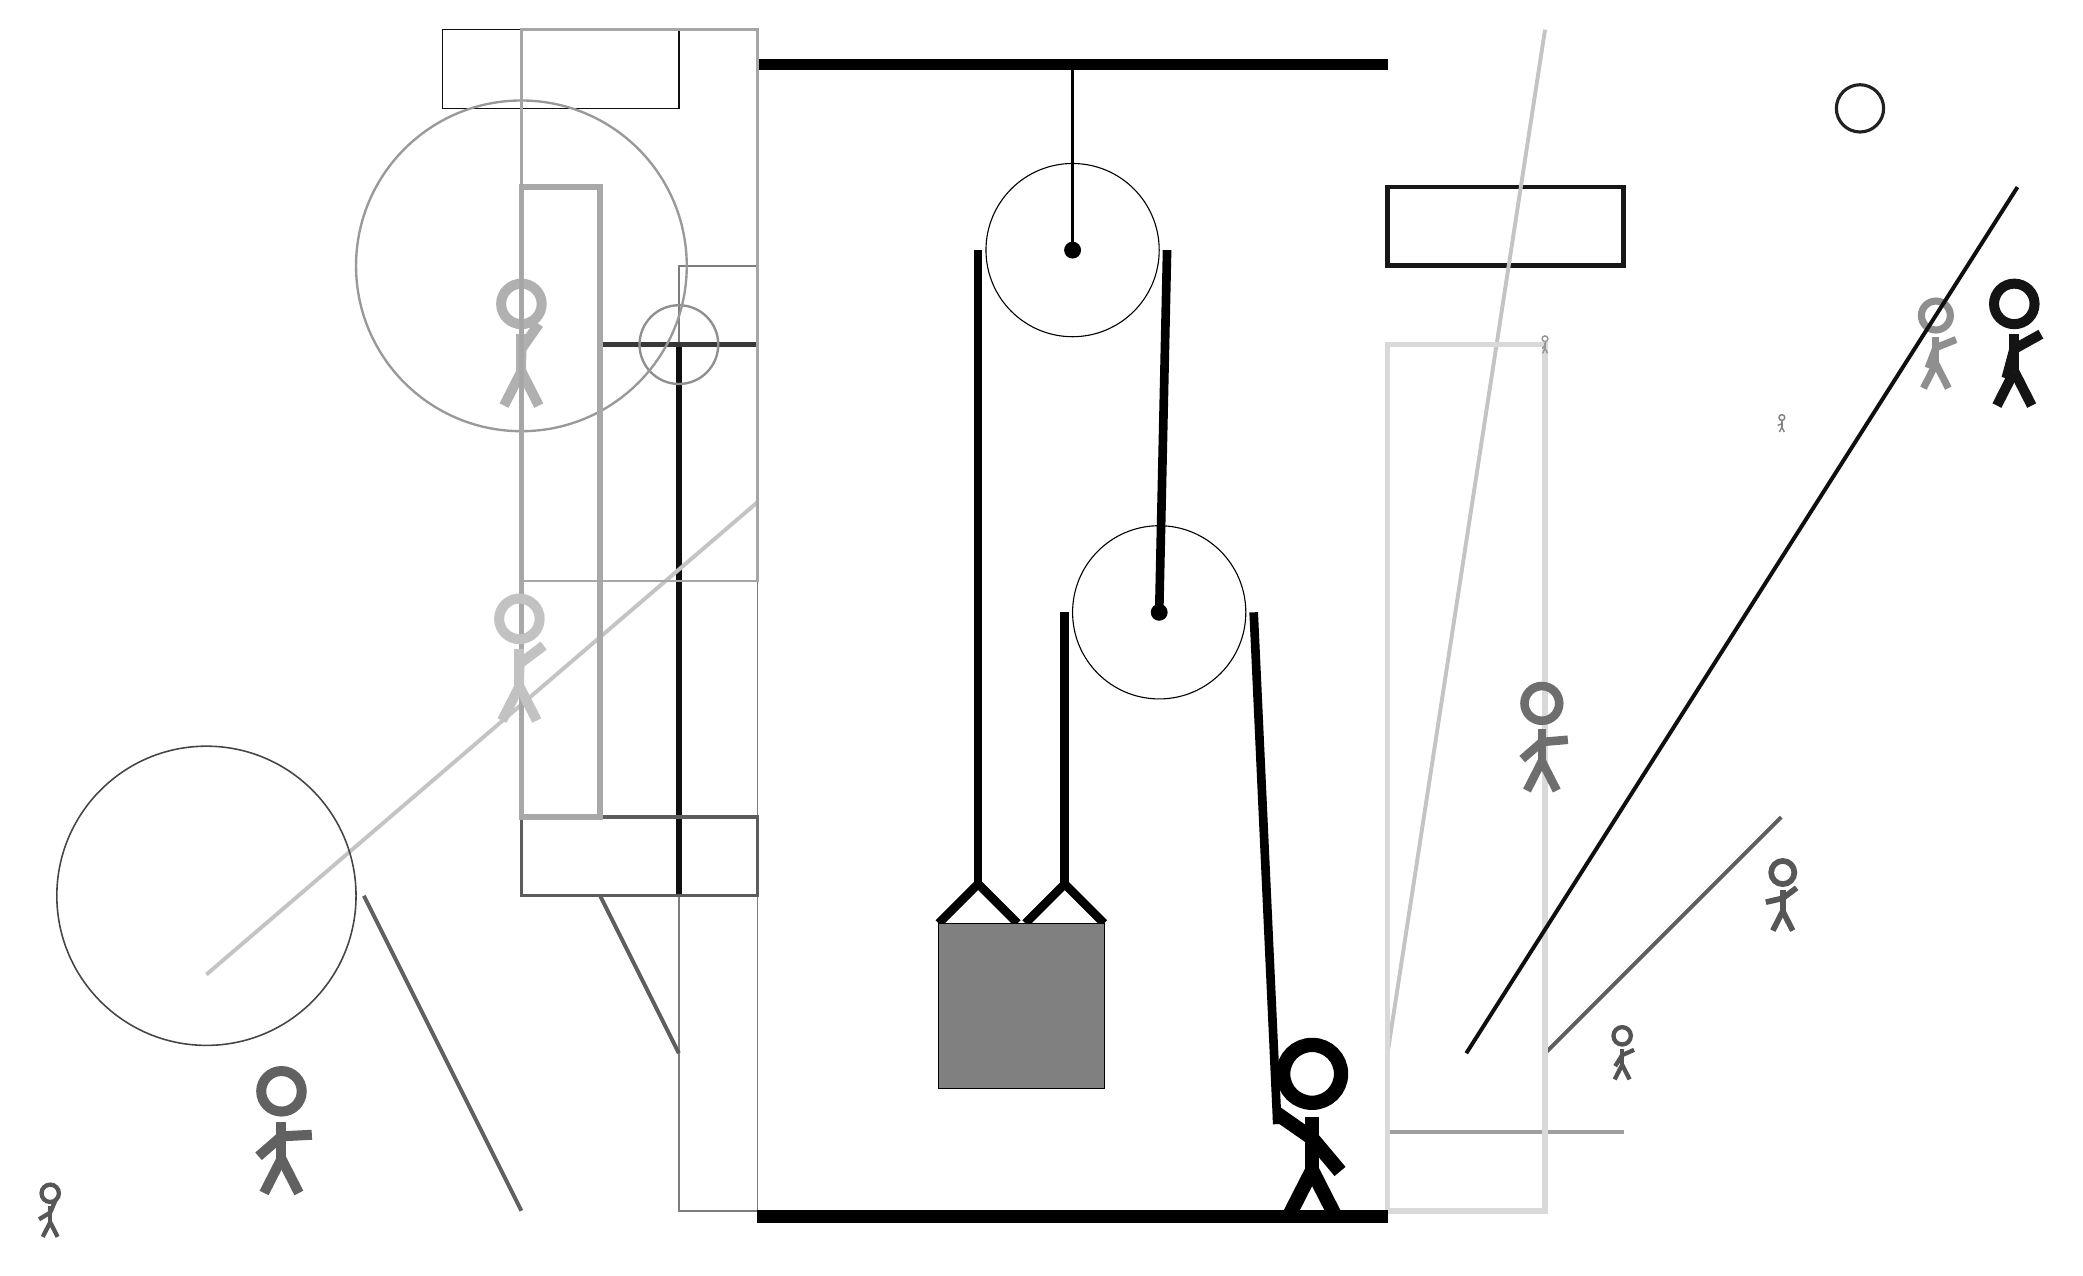
\begin{tikzpicture}
			%%%%% START %%%%%
			
			\draw[fill=black] (-2, 11.5) rectangle (6, 11.625);
			
			\draw[line width=0.6mm, color=black!91] (6, 9) rectangle (9, 10);
			
			\node[line width=0.7mm, color=black!67] at (9, -1) {\Strichmaxerl[3][58][24]};
			\draw[line width=0.5mm, color=black!23](6, -1) -- (8, 12);
			\draw[line width=0.5mm, color=black!63](8, -1) -- (11, 2);
			\draw[line width=0.2mm, color=black!94] (-3, 12) rectangle (-6, 11);
			
			\draw[line width=0.2mm, color=black!51] (-2, 9) rectangle (-3, -3);
			\draw[line width=0.7mm, color=black!94] (-3, 1) rectangle (-3, 8);
			\draw[line width=0.5mm, color=black!63](-4, 1) -- (-3, -1);
			\draw [line width=0.4mm, color=black!95](11, 6) circle (0.0);
			\node[line width=0.6mm, color=black!66] at (-11, -3) {\Strichmaxerl[3][31][67]};
			\draw[line width=0.6mm, color=black!78] (-2, 8) rectangle (-4, 8);
			\draw [line width=0.3mm, color=black!44](-3, 8) circle (0.5);
			\draw[line width=0.5mm, color=black!38](9, -2) -- (6, -2);
			
			\node[line width=0.4mm, color=black!44] at (13, 8) {\Strichmaxerl[5][69][22]};
			\node[line width=0.6mm, color=black!31] at (-5, 8) {\Strichmaxerl[7][89][55]};
			\draw [line width=0.3mm, color=black!40](-5, 9) circle (2.1);
			
			\draw[line width=0.5mm, color=black!23](-2, 6) -- (-9, 0);
			
			\draw[line width=0.4mm, color=black!64] (-2, 2) rectangle (-5, 1);
			\draw[line width=0.5mm, color=black!62](-5, -3) -- (-7, 1);
			\draw[line width=0.7mm, color=black!15] (8, -3) rectangle (6, 8);
			\draw [line width=0.4mm, color=black!87](12, 11) circle (0.3);
			
			\draw[line width=0.7mm, color=black!34] (-4, 10) rectangle (-5, 2);
			\node[line width=0.7mm, color=black!57] at (8, 3) {\Strichmaxerl[6][41][5]};
			\node[line width=0.5mm, color=black!62] at (-8, -2) {\Strichmaxerl[7][41][3]};
			\node[line width=0.6mm, color=black!49] at (11, 7) {\Strichmaxerl[1][18][88]};
			
			\draw[line width=0.3mm, color=black!35] (-2, 12) rectangle (-5, 5);
			\node[line width=0.7mm, color=black!24] at (-5, 4) {\Strichmaxerl[7][89][37]};
			\node[line width=0.6mm, color=black!92] at (14, 8) {\Strichmaxerl[7][75][29]};
			\node[line width=0.5mm, color=black!66] at (11, 1) {\Strichmaxerl[4][13][37]};
			\draw[line width=0.5mm, color=black!94](7, -1) -- (14, 10);
			\draw [line width=0.2mm, color=black!73](-9, 1) circle (1.9);
			
			\node[line width=0.5mm, color=black!41] at (8, 8) {\Strichmaxerl[1][51][79]};
			
			\draw (2, 9.2) circle (1.1);
			\draw[fill=black] (2, 9.2) circle (0.1);
			\draw[thick] (2, 9.2) -- (2, 11.5);
			
			\draw (3.1, 4.6) circle (1.1);
			\draw[fill=black] (3.1, 4.6) circle (0.1);
			
			\draw[line width = 1.1mm]  (0.3, 0.65) -- (0.8, 1.15) -- (1.3, 0.65);
			\draw[line width = 1.1mm]  (1.4, 0.65) -- (1.9, 1.15) -- (2.4, 0.65);
			\draw[fill=black!50] (0.3, 0.65) rectangle (2.4, -1.45);
			
			\draw[line width = 1.1mm] (0.8, 9.2) -- (0.8, 1.15);
			\centerarc[line width = 1.1mm](2, 9.2)(0:180:1.2000000000000002);
			\draw[line width = 1.1mm] (3.2, 9.2) -- (3.1, 4.6);
			\draw[line width = 1.1mm] (1.9, 4.6) -- (1.9, 1.15);
			\centerarc[line width = 1.1mm](3.1, 4.6)(0:180:1.2000000000000002);
			\draw[line width = 1.1mm] (4.3, 4.6) -- (4.6, -1.9);
			
			\node at (5, -2) {\Strichmaxerl[10][-35][-50]};
			
			\draw[fill=black] (-2, -3) rectangle (6, -3.15);
			
			%%%%% END %%%%%
		\end{tikzpicture}
	\end{figure}	
\end{document}